% !TEX encoding = UTF-8
% !TEX TS-program = pdflatex
% !TEX root = ../tesi.tex

%**************************************************************
\chapter{Protocolli di modellazione e trasferimento dati}
\label{protocolli-trasmissione-dati}
%**************************************************************

\intro{Il capitolo tratta i protocolli di modellazione e trasferimento dati dal punto di vista teorico, in particolare viene approfondito lo stile architetturale REST e il linguaggio di query GraphQL.}\\

%**************************************************************
\section{Introduzione ai protocolli}
\subsection{Modello architetturale client-server}
\label{client-server}
Prima di procedere nella spiegazione dei protocolli di trasferimento e modellazione dati, è necessario fare una breve introduzione sull'architettura delle Web Application moderne. Quest'ultime seguono il modello server - client, ovvero un modello architetturale che divide in due processi l'applicazione: un client che richiede servizi al server il quale li esegue ritornando una risposta contenente l'esito dell'operazione. \\\\
I protocolli di trasferimento e modellazione dati trovano il loro maggior utilizzo proprio nella comunicazione server - client; di seguito viene introdotto il concetto di Application Programming Interface necessario per comprendere il funzionamento dei protocolli di data fetching.
\subsection{Application Programming Interface}
 Le API sono interfacce comunemente realizzate per permettere la comunicazione tra server e client. Ciascun applicativo/dispositivo è sviluppato con strutture di dati differenti che evolvono nel tempo, risulta perciò complessa la comunicazione tra di essi. Le API giocano un ruolo fondamentale nello scambio di dati poiché definiscono una interfaccia per la comunicazione; quest'ultima è indipendente dall'implementazione del dispositivo o dell'applicativo e permette di comunicare secondo rispettando regole ben documentate. Risultano dunque fondamentali nella comunicazione, collaborazione e integrazione di nuovi componenti applicativi.\\
 Al giorno d'oggi le API sono utilizzate dalla maggior parte delle Web Application, dispositivi IoT e applicativi di vario genere.\\ \\
 Il documento fa riferimento alle Web API, cioé a quelle interfacce che sfruttano principalmente il protocollo HTTP per la comunicazione server - client. Tra i vari tipi di Web API troviamo:
 \begin{itemize}
   \item \textbf{API pubbliche}: API accessibili da tutti;
   \item \textbf{API private}: API create con lo scopo di essere utilizzate solo ed esclusivamente all'interno dell'azienda;
   \item \textbf{API partner}: API utilizzate tra aziende in collaborazione;
   \item \textbf{API composte}: API differenti combinate tra loro per creare una sequenza di operazioni.
 \end{itemize}
La necessità di standardizzare il modo in cui vengono sviluppate le interfacce API ha portato dunque alla nascita dei protocolli di data fetching.
\subsection{Protocolli di trasferimento dati}
Per protocolli di modellazione e trasferimento dati s'intende un insieme di regole, strutture e vincoli che regolano il corretto funzionamento delle API. Permettono dunque di definire una sorta di standard al quale gli sviluppatori possono far riferimento per implementare e interagire con esse. Il termine protocollo non si addice perfettamente a tutte le varie tecnologie di data fetching, tuttavia a grandi linee può racchiuderle e dunque verrà utilizzato per questione di comodità.
\subsection{I primi protocolli}
Di seguito i più importanti protocolli in uso prima dell'avvento di REST e GraphQL. Si tratta di tecnologie aventi tutte lo stesso scopo, ma di natura completamente differente.
\subsubsection*{Remote Procedure Call}
Il protocollo RPC prevede l'invocazione di una procedura o subroutine del server da parte del client. Il server esegue dunque la logica di business corrispondente senza che il client ne conosca i dettagli. Dal punto di vista del client l'esecuzione avviene localmente, ma in realtà è il server remoto a garantirla.\\
Di seguito riportata la definizione attribuita all'RPC dagli informatici Andrew Birrell e Bruce Nelson nel 1984:
  \begin{quoting}
    \textit{“Meccanismo sincrono che trasferisce il flusso di controllo e i dati attraverso una chiamata di procedura tra due spazi di indirizzo su una rete a banda stretta.”}
  \end{quoting}
Come nelle chiamate a procedure locali, un RPC è una operazione sincrona che tiene in pausa il client fino al momento in cui ritorna il risultato della procedura invocata.
\subsubsection*{Simple Object Access Protocol}
SOAP è un vero e proprio protocollo che definisce la struttura dei dati che devono essere trasferiti ed il modo in cui questi devono essere elaborati. Richiede esclusivamente il formato XML per trasferire dati e tipicamente viene utilizzato il protocollo HTTP per il trasferimento di file, tuttavia possono essere utilizzati anche protocolli differenti come ad esempio il protocollo SMTP. La struttura di un messaggio SOAP è composta da tre principali componenti:
\begin{itemize}
  \item \textbf{Envelope}: necessario al fine di identificare il documento come messaggio SOAP;
  \item \textbf{Header}: opzionale. Il suo scopo è quello di fornire informazioni che vengono interpretate dai moduli di rete durante il trasporto del messaggio;
  \item \textbf{Body}: il body contiene il vero e proprio messaggio che si vuole trasferire.
\end{itemize}
\section{Approfondimento sullo stile architetturale REST}
REST è uno stile architetturale introdotto da Roy Fielding nel 2000 e viene considerato al giorno d'oggi come uno standard per la realizzazione di Web API. Questo stile architetturale prevede l'astrazione degli elementi che compongono il sistema da modellare; di questi elementi REST ignora i dettagli implementativi ed espone esclusivamente gli aspetti necessari per l'interazione con essi; introduce inoltre convenzioni da rispettare nella comunicazione server - client.
\subsection{Principi dell'architettura REST}
\label{principi-REST}
Una interfaccia API è definibile RESTful se rispetta i sei principi indicati da Roy Fielding.
\subsubsection*{Server - client}
Il primo principio sposa uno dei paradigmi cardine dell'informatica: il principio di \textit{Separation of concerns} secondo il quale conviene sempre separare un sistema complesso in moduli distinti, ognuno avente un ruolo ben definito.\\
Ciò viene ripreso nell'architettura REST separando il client dal server; così facendo server e client possono essere implementati in maniera indipendente usando qualsiasi lingua o tecnologia, è sufficiente che siano conformi al prossimo principio detto \textit{Uniform Interface}.
\subsubsection*{Uniform Interface}
Si tratta di un principio fondamentale che caratterizza lo stile architetturale REST. Secondo questo prinpicio l'interazione tra componenti Web come client, server e gli intermediari del network, dipendono dalla uniformità delle loro interfacce.\\
I componenti Web dunque sono in grado di comunicare coerentemente seguendo i seguenti vincoli di interfaccia delineati da Fielding:
\begin{itemize}
  \item \textbf{Identification of resources}: le risorse coinvolte devono essere identificate nella richiesta stessa, dunque specificandole nell'url;
  \item \textbf{Manipulation of resources through representations}: il client non si deve curare di come sono strutturate le risorse all'interno del server, ma deve conoscere la loro rappresentazioni in termini di dati ed utilizzare correttamente i metodi HTTP per manipolarle;
  \item \textbf{Self-descriptive messages}: in ciascun messaggio devono esser presenti le informazioni necessarie a descrivere come deve essere processata la richiesta;
  \item \textbf{Hypermedia as the Engine of Application State}: la rappresentazione dello stato di una risorsa deve includere i riferimenti alle risorse correlate. É dunque necessario includere i link per ciascuna risposta, così che il client possa navigare tra le risorse correlate.
\end{itemize}
\subsubsection*{Layered System}
Secondo questo principio l'architettura di un applicativo deve essere composta da più strati. Ciascuno strato deve ingorare gli altri strati tranne quelli ad esso adiacenti. Questi layer possono essere composti da intermediari basati sul network i quali intercettano la comunicazione server - client con uno scopo specifico (ad esempio per questioni di sicurezza, caching, controllo del flusso dati, ecc...), possono essere ad esempio proxy e gateways. Per il principio di Layered System questi intermediari devono aderire alle interfacce al fine di mantenerne l'uniformità.
\subsubsection{Cache}
Si tratta di uno dei vincoli fondamentali in un archiettura Web, secondo il quale un web server deve etichettare i dati di ogni risposta come adatti o meno alla permanenza in cache. Così facendo gli intermediari tra server e client e il client stesso sanno come comportarsi riguardo alla memorizzazione in cache dei dati ritornati.
\subsubsection{Stateless}
Il vincolo di stateless fa riferimento al fatto che un server non deve memorizzare lo stato dell'applicazione client. Questo implica però che ogni richiesta che il server riceve dal client deve essere sufficientemente dettagliata sullo stato del client affinché il server sia in grado di eseguirla. Dunque le richieste non sono correlate tra loro e per questo tale comunicazione viene definita priva di stato. \\
Questo vincolo porta un vantaggio fondamentale secondo il quale un server così facendo può gestire richieste da molti client. Può inoltre esser scalato molto più facilmente con l'aiuto ad esempio di un load balancer.
\subsubsection{Code on demand}
Per ultimo troviamo il vincolo di code on demand. Si tratta di un vincolo facoltativo secondo il quale il server può inviare al client della logica da eseguire localmente.
\section{Approfondimento sul linguaggio di query GraphQL}
\subsection{Introduzione}
GraphQL è stato ideato da Facebook nel 2012 e condiviso e reso pubblico nel 2014. Al giorno d'oggi molte importanti applicazioni utilizzano GraphQL come ad esempio GitHub, Twitter, PayPal e Pinterest. Viene considerato come il principale competitor e possibile successore di REST nell'ambito del data fetching tuttavia, come verrà spiegato in seguito, oltre a svariati punti di forza e di innovazione ha anche alcune debolezze.\\
Più nello specifico GraphQL è un linguaggio di query. Viene definito agnostico rispetto al mezzo di trasporto perché non dipende dal modo in cui client e server comunicano, ma solitamente viene utilizzato sul protocollo HTTP. Il principale punto di forza di GraphQL è la possibilità di specificare nella query esattamente i dati che si è interessati a ricevere, questo permette di non occupare la rete per dati non richiesti. Altro importante punto di forza, ma che talvolta può risultare un problema, è che è fortemente tipizzato.\\
Affermare che GraphQL abbia lo scopo di servire esclusivamente come linguaggio di query può risultare riduttivo. Uno dei principali motivi d'utilizzo di GraphQL è quello di riuscire a raggruppare tutti i dati e servizi di un'applicazione insieme in uno stesso posto e fornire così un'interfaccia unica che risulti consistente, sicura e infine semplice da utilizzare.\\
GraphQL non specifica come deve essere costruita un'API, tuttavia ci sono cinque linee guida dette "Principi di desing" da tenere in considerazione durante lo sviluppo:
\begin{itemize}
  \item \textbf{Hierarchical}: i tipi ricercati in una query GraphQL seguono una struttura gerarchica; i tipi possono avere come campi altri tipi e così via. Inoltre i dati che vengono ritornati dalla query, vengono ritornati esattamente con la medesima struttura con cui sono stati richiesti;
  \item \textbf{Product centric}: le API sono inevitabilmente guidate dalle richieste del client, per questo bisogna realizzarle in maniera flessibile cercando di tener conto delle possibili richieste client;
  \item \textbf{Strong typing}: un server GraphQL è supportato da un type system specifico a seconda dell'applicazione. Data una query il server assicura che questa sia sintatticamente corretta, valida e che i tipi in gioco rispettino esattamente la struttura dei tipi definiti nel GraphQL schema;
  \item \textbf{Client-specified queries}: in GraphQL la codifica della query avviene nel client e non nel server e si tratta di query che vanno a specificare campo per campo. Nella maggior parte dei sistemi che non utilizzano GraphQL il server determina quali dati ritornare. In GraphQL ciò non accade, vengono infatti ritornati solo i dati specificati dal client;
  \item \textbf{Introspective}: GraphQL è introspettivo, infatti i client possono consultare a fondo il GraphQL Schema e possono dunque vedere tutte le query disponibili, i vari tipi e i loro campi.
\end{itemize}
\subsection{GraphQL schema}
GraphQL ha cambiato il modo di pensare alle API: queste non vengono più considerate come un insieme di endpoints dai quali ottenere dati ed eseguire servizi, ma vengono piuttosto considerate come una collezione di tipi e relazioni distribuiti su grafo. Questa collezione di tipi e loro relazioni deve essere riportata in maniera chiara in una pagina chiamata \textbf{GraphQL Schema}. In questo schema devono essere definiti tutti quei tipi che si vuole esporre alle richieste del client per esser modificati, aggiunti, eliminati o semplicemente visualizzati. Il GraphQL schema viene realizzato con un linguaggio denominato SDL (Schema Definition Language) il quale permette di specificare le operazioni disponibili, i tipi e le relazioni tra di essi.\\
Durante la progettazione e la realizzazione di un server di backend possono essere seguite due differenti tecniche per implementare schema e codice:
\begin{itemize}
  \item \textbf{Schema first}: questa tecnica si discosta dal classico ordine di realizzazione di un server di backend infatti, come deducibile dal nome, prevede la realizzazione del GraphQL Schema prima di realizzare i resolver delle API;
  \item \textbf{Code first}: questa tecnica è opposta alla precedente in quanto prevede la realizzazione prima dei resolver e solo in seguito dello schema.
\end{itemize}
Non è chiaro quale delle due tecniche sia migliore, sono aperti ancora diversi dibattiti a riguardo, in questo progetto è stato seguito il modello Schema first durante la migrazione.\\
Grazie alla presenza del GraphQL Schema gli sviluppatori frontend sono in grado di conoscere nel dettaglio la struttura di ciascun tipo e delle varie operazioni disponibili. Le API sviluppate con GraphQL si autodocumentano: è sufficiente la consultazione dello schema per comprendere la natura delle entità che si desidera interrogare o manipolare.
\subsection{Definizione dei tipi}
Come già evidenziato GraphQL è un linguaggio di query fortemente tipizzato. I tipi sono l'unità principale di un GraphQL Schema.\\
Per tipo si intende un oggetto costruito campo per campo e dovrà poi corrispondere ad una entità nel backend dell'applicativo. All'interno dello schema compaiono tutti i tipi che andranno a rappresentare la struttura dati dell'applicativo.\\
Un tipo può contenere come campi dati altri tipi definiti nel medesimo schema. Di seguito l'esempio della dichiarazione del tipo \textit{Employee}:
\begin{verbatim}
  type Employee {
    id: ID
    name: String!
    owns: Badge
    worksIn: Department
    worksOn: [Project]
    ...
  }
\end{verbatim}
In questo caso il tipo Employee è composto dai campi:
\begin{itemize}
  \item \textbf{id}: un codice identificativo di tipo \textit{ID};
  \item \textbf{name}: un nome di tipo \textit{String}, il punto esclamativo indica che si tratta di un campo che non può essere nullo;
  \item \textbf{owns}: un badge di tipo \textit{Badge} per l'accesso al dipartimento;
  \item \textbf{worksIn}: un dipartimento di tipo \textit{Department} nel quale lavora l'impiegato;
  \item \textbf{worksOn}: una lista di progetti di tipo \textit{Project} al quale l'impiegato sta lavorando.
\end{itemize}
I tipi \textit{Department}, \textit{Badge} e \textit{Project} devono essere necessariamente definiti all'interno dello stesso GraphQL schema di Employee.\\
I built-in type che GraphQL mette a disposizione vengono detti \textbf{scalar-type} e sono: \textit{Int}, \textit{String}, \textit{Boolean}, \textit{ID}, \textit{Float}.\\
È possibile inoltre dichiarare anche degli scalar-type personalizzati con la keyword "\textit{scalar}", oppure delle enumerazioni attraverso l'utilizzo della keyword "\textit{enum}". Infine è prevista anche l'unione tra più tipi tramite la kewyword "\textit{union}" come segue:
\begin{lstlisting}[language=GraphQL,]
  union worker = Employee | Manager | Chief
\end{lstlisting}
In questo caso sono stati uniti in un unico tipo \textit{worker} i tipi \textit{Employee}, \textit{Manager} e infine \textit{Chief}.
3ex{Connessioni tra tipi}
GraphQL è cosi denominato perché oltre ad essere un Query Language come suggeriscono le ultime due lettere del nome, permette di definire connessioni di vario genere tra i tipi definiti nello schema, queste connessioni vanno di fatto a creare uno grafo composto da tipi interconnessioni, da questo deriva il prefisso \textit{Graph}.
È fondamentale durante la definizione del GraphQL Schema riportare le relazioni tra tipi in modo consistente. \\
In GraphQL risulta essere una buona pratica dare bidirezionalità alle connessioni ove possibile, questo con lo scopo di lasciare flessibilità allo sviluppatore client il quale da una query specifica può raggiungere diversi tipi e spostarsi nel grafo come più desidera.\\
Di seguito vengono elencate le varie relazioni con relativi esempi.
\subsubsection*{Connessione one-to-one}
Nelle relazioni one-to-one ad un tipo viene associata una sola istanza di un altro tipo e viceversa. Riprendendo il caso del tipo Employee riportato sopra, possiamo trovare una relazione del tipo one-to-one tra i tipi Employee e Badge. Di seguito la rappresentazione del grafo:
\begin{figure}[!h]
\centering
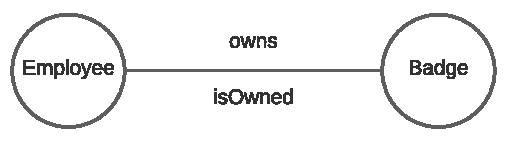
\includegraphics[width=0.5\linewidth]{immagini/one_to_one.pdf}
\caption{Connessione one-to-one}
\label{one-to-one}
\end{figure}
\\ \\
Come mostrato in figura \ref{one-to-one} il collegamento tra i due tipi è definito come "owns" se si legge nel verso che parte da Employee per raggiungere Badge e fa riferimento all'omonimo campo di Employee. Se altrimenti la connessione si percorre nel verso opposto viene definita "isOwned", come l'omonimo campo di Badge, riportato in seguito:
\begin{lstlisting}[language=GraphQL,]
  type Badge {
    id: ID
    isOwned: Employee
    ...
  }
\end{lstlisting}
\subsubsection*{Connessione one-to-many}
In questo caso bisogna focalizzarsi sul campo \textit{worksIn} di Employee. Questo campo definisce la connessione con un elemento di tipo \textit{Department}, dunque a ciascun impiegato corrisponde un dipartimento nel quale lavora. Tuttavia pensando alla connessione in senso opposto a ciascun dipartimento possono corrispondere più impiegati. Segue dunque la rappresentazione della connessione nel grafo:\\

\begin{figure}[!h]
\centering
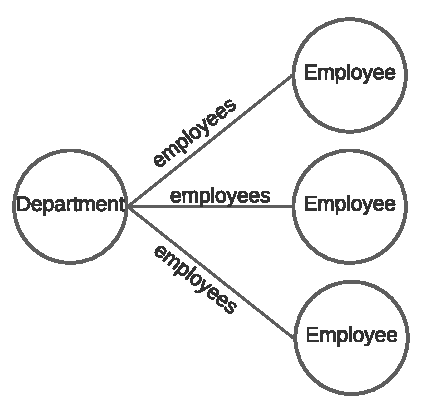
\includegraphics[width=0.4\linewidth]{immagini/one_to_many.pdf}
\caption{Connessione one-to-many}
\label{one-to-many}
\end{figure}
\mbox{}\\
Come mostrato in figura \ref{one-to-many} il collegamento tra il dipartimento e i vari impiegati viene chiamato "employees" se si considera il verso che parte da Department per raggiungere Employee e corrisponde all'omonimo campo di Department. Volendo è possibile attribuire doppia direzionalità alla relazione. Di seguito il tipo Department con il campo "employees":
\begin{lstlisting}[language=GraphQL,]
  type Department {
    id: ID
    name: String!
    address: String!
    employees: [Employee]
  }
\end{lstlisting}
\subsubsection*{Connessione many-to-many}
Consideriamo ora il campo \textit{worksOn} di Employee che collega ciascun impiegato con una lista di progetti ai quali sta lavorando. In questo caso considerando il collegamento nel verso opposto anche ciascun progetto può avere più impiegati che ci lavorano. In questo caso si tratta di una relazione many-to-many e segue la rappresentazione nel grafo:
\begin{figure}[!h]
\centering
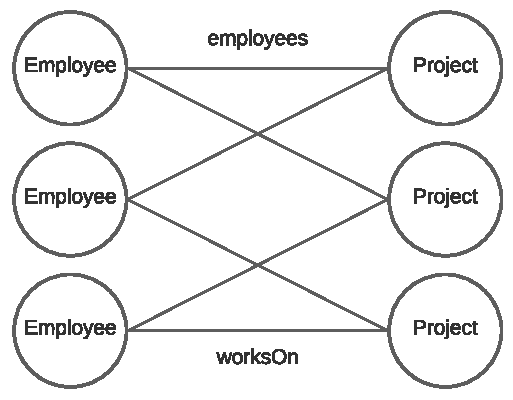
\includegraphics[width=0.4\linewidth]{immagini/many_to_many.pdf}
\caption{Connessione many-to-many}
\label{many-to-many}
\end{figure}
Le relazioni many-to-many non sono altro che l'unione di due relazioni one-to-many.
La connessione in questo caso, come nei casi precedenti, a seconda del verso in cui viene percorsa può esser definita come "worksOn" o "employees" come mostrato in figura \ref{many-to-many}. Di seguito la rappresentazione del tipo Project:
\begin{lstlisting}[language=GraphQL,]
  type Project {
    id: ID
    name: String
    employees: [Employee]
  }
\end{lstlisting}
\subsection*{Operazioni sui dati}
Ci sono tre tipi di operazioni che possono essere eseguite sui dati: \textit{Query}, \textit{Mutation} e \textit{Subscription}.
\subsubsection{Query}
L'operazione di query viene utilizzata per richiedere dati da una determinata API ed equivale alla GET nel protocollo REST. È necessario dichiarare nel GraphQL Schema la query che il programmatore backend desidera rendere disponibile, così facendo vengono dichiarati anche i tipi che possono eventualmente essere passati come argomenti e quelli che verranno ritornati dalla query.\\
Un esempio di dichiarazione di query che ritorna una lista di tutti gli oggetti di tipo Employee presenti in un determinato Department può essere:
\begin{lstlisting}[language=GraphQL,]
  type query {
    employeesInDepartment(departmentId: ID!): [Employee]
  }
\end{lstlisting}
In questo caso invocando la query \textit{employeesInDepartment} e passando come argomento l'id del dipartimento riceveremo come risposta un JSON contenente un campo "\textit{data}" che presenterà al suo interno la lista di impiegati. In caso di insuccesso verrà ritornato un JSON con un campo "\textit{error}" contenente la descrizione dell'errore.\\
Se il client desiderasse invocare la query definita, dovrebbe invocarla nel seguente modo:
\begin{lstlisting}[language=GraphQL,]
  query {
    employeesInDepartment(id: "2BR4S") {
      id
      name
      worksOn {
        id
        name
      }
    }
  }
\end{lstlisting}
In caso di successo verrà ritornata una lista di impiegati per ognuno dei quali compariranno i campi specificati nella query: \textit{id}, \textit{name}, \textit{worksOn}. \textit{worksOn} contiene la lista di progetti per ognuno dei quali verranno indicati esclusivamente i campi: \textit{id}, \textit{name}.\\
La tecnica \textit{data paging} consente di realizzare meccanismi personalizzati di paginazione specificando la numerosità delle ricorrenze desiderate tramite appositi parametri previsti nella query.
\subsubsection*{Mutation}
L'operazione di mutation viene utilizzata per eseguire modifiche sui dati. Equivale all'unione delle operazioni POST, DELETE e PUT utilizzate in REST. Come per le query è necessario dichiarare le mutation che si vogliono rendere disponibili al client.\\
Un esempio di mutation può essere:
\begin{lstlisting}[language=GraphQL,]
  type mutation {
    addNewEmployee(employee: Employee!): Employee
  }
\end{lstlisting}
In questo caso la mutation \textit{addNewEmployee} andrà ad aggiungere un nuovo impiegato nell'archivio dell'applicativo. Il client per invocare questa mutation dovrà strutturare la richiesta come segue:
\begin{lstlisting}[language=GraphQL,]
  mutation {
    addNewEmployee(employee: {
      name: "Mario"
    }){
      id
    }
  }
\end{lstlisting}
In questa mutation è stato passato come argomento un oggetto di tipo Employee di cui è stato specificato esclusivamente il nome. La definizione della mutation prevede il ritorno di un oggetto di tipo Employee. In questo caso il client dichiara di essere interessato esclusivamente all'id dell'impiegato appena creato.
\subsubsection*{Subscription}
L'ultimo tipo si chiama Subscription e si tratta di una funzione particolare resa disponibile in GraphQL. Grazie a questa funzione i client possono dichiarare il loro interessa ad una subscription; il client non è costretto ad eseguire polling poiché, al verificarsi della condizione, sarà il server ad avvertire il client.\\
Un esempio di definizione di una Subscription può essere:
\begin{lstlisting}[language=GraphQL,]
  type subscription {
    newEmployeeAdded: Employee!
  }
\end{lstlisting}
Il client che desidera sottoscriversi alla subscription \textit{newEmployeeAdded} dovrà mandare una richiesta strutturata come segue:
\begin{lstlisting}[language=GraphQL,]
  subscription {
    newEmployeeAdded {
      id
      name
    }
  }
\end{lstlisting}
Così facendo il server, appena viene aggiunto un nuovo impiegato, invierà direttamente al client i dati che il client ha specificato nella sottoscrizione, in questo caso \textit{id} e \textit{name} dell'impiegato.\\
Essendo il server a dover inviare i dati al client e non viceversa, non sarà utilizzato il protocollo HTTP per la comunicazione server - client bensì il protocollo WebSocket che aprirà un canale di comunicazione a doppia via sopra un socket TCP.\
